\documentclass[a4paper]{IEEEtran}

% Packages
\usepackage{siunitx}
\usepackage{tikz}
\usepackage{graphicx}
\usepackage{url}
\usepackage{booktabs}
\usepackage{tabu}
\usepackage{multirow}
\usepackage{listings}
\usepackage{ragged2e}

% Use font weights in text for siunitx
\sisetup{detect-weight=true, detect-family=true}

% Listings settings
\lstset{
  frame=single,
  basicstyle=\scriptsize,
  breaklines=true,
  postbreak=\mbox{$\hookrightarrow$}\space,
  numbers=left,
  numbersep=5pt,
  xleftmargin=2em
}

% Code and drawings commands
\newcommand{\srbsource}[2]{
\subsection{\texttt{\protect\url{#1}}}
\lstinputlisting[language=#2]{../#1}
}

\newcommand{\srbdrawing}[3][0.89]{
\subsection{#2}
\noindent
\centering
\includegraphics[height=#1\textwidth, angle=90]{#3}
\justify
}

% NMEA spec environment
\newenvironment{nmeaspec}[1]
{
\newcommand{\field}[2]{\texttt{##1} & ##2 \\}
\vspace{0.2cm}
\noindent\texttt{#1}
\vspace{0.2cm}

\noindent Where: \vspace{0.1cm}\\  \noindent
\vspace{0.2cm}
\begin{tabular}{ll}
}
{
\end{tabular}
}

% Title, author, etc.
\title{\vspace{5.0cm}Autonomous surf life saving device}
\author{\Large Jarod Lam\\ \textit{Supervisor: Matthew Dunbabin}}
\IEEEspecialpapernotice{2018-2019 VRES project at Queensland University of Technology}

\begin{document}

% Title page
\begin{minipage}{\textwidth}
\vfill
\maketitle
\vfill
\end{minipage}
\clearpage

\begin{abstract}
build boat that saves people
\end{abstract}

\tableofcontents

\section{Introduction}
Surf life savers regularly patrol beaches to help those in danger and are essential to keeping public beaches safe. In Queensland alone, over three thousand are rescued and hundreds are resuscitated by lifesaving services every year. \cite{lifesaving} Even so, from 2008-2018, there was an average of 47 drowning deaths per year at Australian beaches--a tragically high number that many organisations are working to reduce. \cite{drowning}

To supplement the activities of surf life savers and other services at public beaches, a system has been proposed that will allow timely help to be given to people in distress while waiting to be rescued. The surf rescue boat (SRB) aims to deliver help quickly and reduce the risk to which life savers are exposed.

The basic concept of the design is a remotely-controlled floating water vehicle that sits in the surf away from the shore at a beach. At most times, the vehicle is idle and remains stationary in the surf. When a person in distress is seen, a life saver on the shore can remotely direct the vehicle to the person to support them while they wait for help.

A simple water-based robot such as the one proposed can be constructed relatively cheaply and easily with off-the-shelf components. In the future, systems such as these may become widely available and save the lives of many along coastal beaches.

The system is divided into three main sections: the remotely operated water vehicle (the "boat"), an XBee-based radio communications system between the boat and a base station, and a computer vision-based control system. Out of these, only the vehicle and communications were prototyped in this project; the control system has been developed separately in the past and time constraints prevented it from being implemented.

Design considerations taken into account include cost of construction, parts, and maintenance; usability and user-friendliness; and effectiveness as a water-based vehicle.

This report describes these systems in detail, the design and testing methodology, and avenues that can be explored for future development of the surf rescue boat.

\section{Boat}

\subsection{Mechanical}
The remotely operated boat uses a standard surfboard as a base, and houses electronics in a watertight hard plastic case attached to the top. Two propellers are mounted to the bottom of the surfboard for movement control.

\subsubsection{Chassis}
Surfboard. Chosen for its stability and familiarity in the surf. The standardness and availability of surfboards is an advantage to encouraging development of such systems. A custom-built chassis may have been designed, but would have taken more time and money. 

\subsubsection{Propellors}
2 Blue Robotics T100 Thrusters. A propeller is mounted each to the left and right of the surfboard's middle underside. Aluminium mounting plates, attached to the board with Sikaflex, were designed to distribute force and allow propellors to be detached easily.

\subsubsection{Electronics housing}
Pelican 1120 Case. A laser-cut acrylic frame was made to mount the electronics in the box. Wire glands on the side of the box allow propellor wires to be fed through the box walls.

\subsection{Electronics}
An Arduino Mega 2560 controls the onboard electronics mounted in the case. GPS and IMU modules are used for navigation, and an XBee radio communicates with the base station. Two electronics speed controllers (ESCs) control each of the two propellers. A block connection diagram of the electronics is shown in Figure \ref{elecdiag}.

\begin{figure}
\center
\pgfdeclarelayer{bg}
\pgfsetlayers{bg,main}
\begin{tikzpicture}

% Arduino
\draw [fill=teal!50] (0,0) rectangle ++(3,3) node [pos=0.5, align=center] (A) {Arduino Mega};

% Batteries
\draw [fill=blue!50] (A)++(-2.5,4.5) rectangle ++(1,-2) node [pos=0.5, rotate=90] (B1) {Battery 1};
\draw [fill=blue!50] (A)++(-1,4.5) rectangle ++(1,-2) node [pos=0.5, rotate=90] (B2) {Battery 2};

% ESCs
\draw [fill=yellow!50] (A)++(-3.5,-4.5) rectangle ++(0.5,2) node [pos=0.5, rotate=90] (E1) {ESC 1};
\draw [fill=yellow!50] (A)++(-2.5,-4.5) rectangle ++(0.5,2) node [pos=0.5, rotate=90] (E2) {ESC 2};

% XBee
\draw [fill=red!50] (A)++(1,4.5) rectangle ++(2,-2) node [pos=0.5] (X) {XBee};

% GPS
\draw [fill=green!80!black!20!white] (A)++(-1.5,-4.5) rectangle ++(2,2) node [pos=0.5] (G) {GPS};

% IMU
\draw [fill=red!50] (A)++(1,-4.5) rectangle ++(2,2) node [pos=0.5] (I) {IMU};

\begin{pgfonlayer}{bg}

% Power lines
\draw [red, thick] (E2)++(0.25,1) -- (B1) node [pos=0.5, rotate=90, above] {11.1V};
\draw [red, thick] (E1)++(0.25,1) -- ++(0,1.25) -- ++(1,0);
\draw [red, thick] (B2) -- ++(0,-1.5) -- ++(-1.5,0);
\draw [red, thick] (A) -- ++(-2,0);

% UART lines
\draw [blue, thick] (G) -- ++(0,2.75) node [pos=0.5, rotate=90, below] {UART};
\draw [blue, thick] (I) -- ++(0,1.5) -- ++(-1.5,0) node [pos=0.5, above] {UART} -- ++(0,1);
\draw [blue, thick] (X) -- ++(0,-1.5) -- ++(-1.5,0) node [pos=0.5, above] {UART} -- ++(0,-1);

% PWM lines
\draw [olive, thick] (E2)++(-0.25,1) -- ++(0,0.3) -- ++(1.5,0) -- ++(0,1);
\draw [olive, thick] (E1)++(-0.25,1) -- ++(0,0.5) -- ++(2.25,0) node[pos=0.45, above] {PWM} -- ++(0,1);

\end{pgfonlayer}

\end{tikzpicture}

\caption{Connection block diagram for onboard electronics.}
\label{elecdiag}
\end{figure}

\begin{figure}
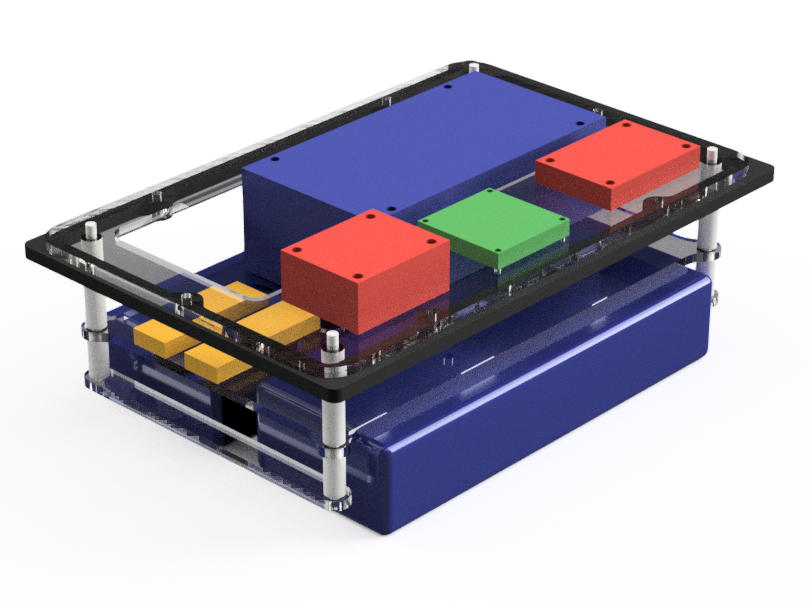
\includegraphics[width=\columnwidth]{assembly.png}
\caption{Rendering of internal electronics frame}
\label{elecframe}
\end{figure}

\begin{figure}[h!]
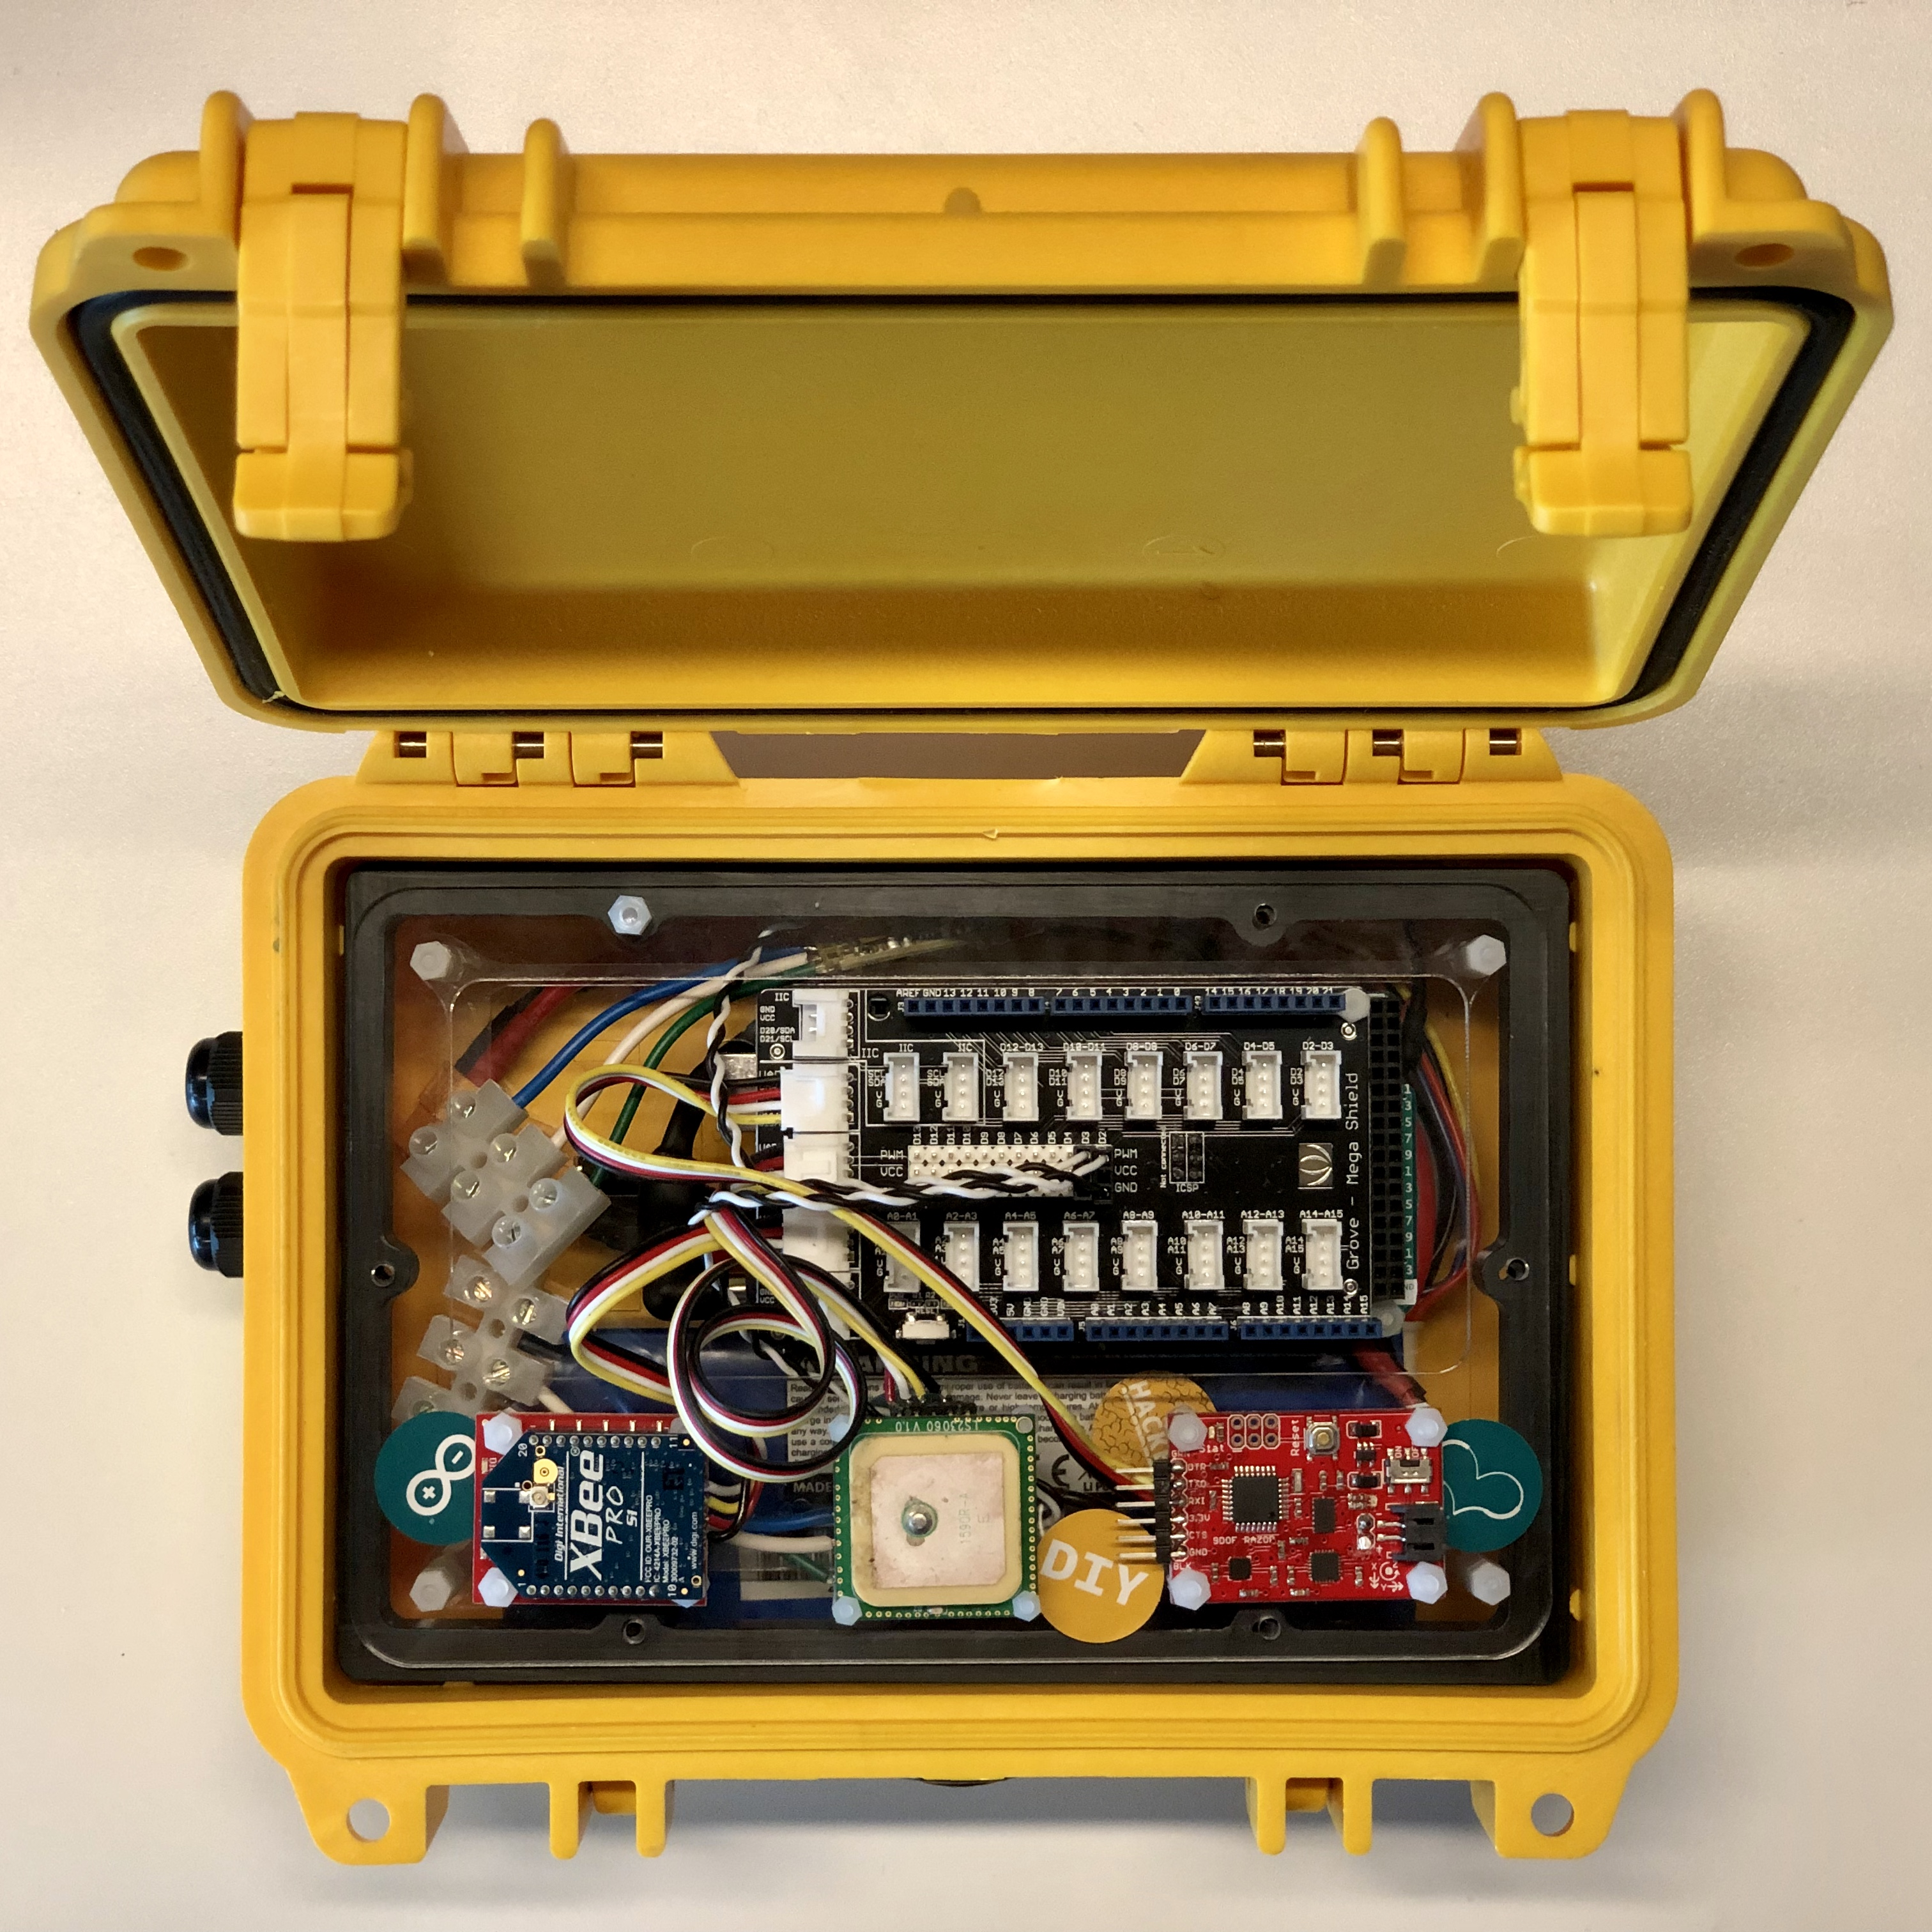
\includegraphics[width=\columnwidth]{boat-hardware.jpg}
\caption{Boat electronics in Pelican case housing}
\label{boathardware}
\end{figure}

\subsubsection{Microcontroller}
Arduino Mega 2560 with Seeedstudio Grove Mega Shield breakout board. This development board is powerful enough to handle relatively simple communication and processing tasks required to control the boat's sensors and motors. More powerful ARM-based boards such as the Raspberry Pi are less suited to rugged environments, and more difficult to recover from failures. The shield provides robust headers to the UART functions of the Arduino.

\subsubsection{Radio}
Digi XBee Pro S1 on a SparkFun XBee Explorer Regulated. This connects to the Arduino via UART, and creates a wireless serial connection to the base station. The protocol is defined in section 3.

\subsubsection{GPS}
LOCOSYS LS20031 GPS receiver. Sends data to the Arduino via UART using the NMEA 0183 protocol found in section 3. 

\subsubsection{IMU}
Sparkfun SEN-10736 9DOF Razor IMU. Sends data to the Arduino via UART. Currently, only the compass value from the sensor is used. Flashed with the Razor AHRS firmware: \url{https://github.com/Razor-AHRS/razor-9dof-ahrs}

\subsubsection{Motor control}
2 Flycolor Raptor 390 30A ESC. Firmware modified to allow forward and backward propeller movement. Receives PWM control signals from the Arduino with a duty cycle range of \SIrange{1000}{2000}{\micro\second}.

\subsubsection{Battery}
2 Zippy Flightmax Z58003S-30 \SI{5800}{mAh} 3S1P. The two batteries are wired in parallel, with a combined nominal capacity of \SI{11.6}{Ah} and nominal voltage of \SI{11.1}{V}.

\subsection{Software}
The Arduino Mega 2560 is programmed in C++ on top of Arduino default and custom libraries. Efforts were made to keep the code somewhat portable and reusable.

The code is split up into several modules, each handling a section of robot operation. These are described below, and the full code can be found in appendix A.

\subsubsection{\texttt{srb}}
Contains the main loop of the program. Initialises values, classes, etc. Runs update functions for GPS, comms, IMU, nav, and motors. Sends \texttt{SRBSM} message at intervals. An AVR watchdog timer is set to reset the microcontroller at the hardware level if the program hangs and reaches a timeout. 

\subsubsection{\texttt{nmea}}
Defines the \texttt{Nmea} class, which contains functions for constructing and parsing NMEA 0183 sentences. This includes generating and validating checksums, counting the number of fields, appending strings and decimal numbers to a sentence, and parsing a sentence by field. All functions use standard C string libraries, so they do not rely on Arduino libraries and will work outside the Arduino environment. Used by \texttt{SrbGps} and \texttt{SrbComms}.

\subsubsection{\texttt{srb\_stats}}
Defines the \texttt{SrbStats} class, which stores the ID, state, GPS and target location, compass and target heading, and other information related to the current state and navigation of the boat. A pointer to the same instance of this class is passed to most other classes when they are created so that they can read and update this information.

\subsubsection{\texttt{srb\_serial}}
Defines the \texttt{SrbSerial} class, which buffers a hardware serial stream and parses the input when a newline is received. The serial port used is configured when the object is created. This is the base class for \texttt{SrbGps}, \texttt{SrbComms}, and \texttt{SrbImu}.

\subsubsection{\texttt{srb\_gps}}
Defines the \texttt{SrbGps} class, which receives and parses GPS fix data over serial. Latitude, longitude, magnetic variation, and ground speed are parsed from the NMEA \texttt{GPRMC} sentence and stored in the \texttt{SrbStats} object. Conversions are made from knots to metres per second, and degrees/minutes to decimal degrees.

\subsubsection{\texttt{srb\_comms}}
Defines the \texttt{SrbComms} class, which sends and receives messages to and from the base station via the XBee radio. Contains functions for constructing and parsing the proprietary NMEA sentences defined in section 3. Stores information and instructions received in the \texttt{SrbStats} object. Stops the boat if no message is received within a timeout period.

\subsubsection{\texttt{srb\_imu}}
Defines the \texttt{SrbImu} class, which receives data from the Sparkfun IMU over serial. Extracts the compass heading from the serial stream and stores it in the \texttt{SrbStats} object.

\subsubsection{\texttt{srb\_motor}}
Defines the \texttt{SrbMotor} class, which controls motor movement. Receives motor power ranges from -100 to 100 and sets the corresponding PWM duty cycle. Accelerates motors to the desired speed at a safe pace.

\subsubsection{\texttt{srb\_nav}}
Defines the \texttt{SrbNav} class, which controls robot navigation. In manual mode, sets motor speed and orients the boat according to target speed and heading sent from the base station. In auto mode, moves the boat toward a set of coordinates sent from the base station. Motors are controlled with the \texttt{SrbMotor} class.

\section{Communications}
Communications between the SRB and the base station are achieved using XBee radios. By attaching a pair of XBee modules to the base station computer and the on-board Arduino, a virtual serial connection is created between the two devices.

\subsection{NMEA 0183 sentences}
NMEA 0183 is a communications specification designed to create a standardised serial interface for GPS devices. Every NMEA `sentence' begins with a \texttt{\$} and ends with \texttt{*CS\textbackslash r\textbackslash n}, where \texttt{CS} is a two-digit hexadecimal checksum of the sentence. Some advantages of using NMEA sentences are that they are standardised, human-readable, robust, and relatively simple to implement. 

A common NMEA sentence type is \texttt{GPRMC}, the GPS recommended minimum. This sentence is used to receive information from the onboard GPS module. \texttt{GPRMC} sentences are specified as follows: \cite{gpsinfo}

\begin{nmeaspec}{\$GPRMC,<Time>,<Status>,<Lat>,<LatDir>,\\<Lon>,<LonDir>,<Speed>,<Angle>,<Date>,\\<MagVar>,<MagDir>*CS}
\field{<Time>}{UTC timestamp in HHmmss format}
\field{<Status>}{Status \texttt{A}=active, \texttt{V}=void}
\field{<Lat>}{Latitude in ddmm.mmm format}
\field{<LatDir>}{\texttt{N} or \texttt{S} hemisphere}
\field{<Lon>}{Longitude in dddmm.mmm format}
\field{<LonDir>}{\texttt{E} or \texttt{W} hemisphere}
\field{<Speed>}{Ground speed in knots}
\field{<Angle>}{Track angle in degrees from north}
\field{<Date>}{Date in DDMMYY format}
\field{<MagVar>}{Magnetic variation magnitude}
\field{<MagDir>}{Magnetic variation direction}
\end{nmeaspec}

A NMEA sentence parser and constructor was written in C++ and Python for the boat and the base station, respectively. Specified below is a set of custom NMEA sentence types that was created for communication between the boat and the base station over the XBee radios.

\subsubsection{\texttt{SRBSM} - Status Message}
The \texttt{SRBSM} sentence is sent periodically by the boat to update the base station with status information.

\begin{nmeaspec}{\$SRBSM,<ID>,<State>,<Lat>,<Lon>,<Speed>,\\<Heading>,<BattV>,<FwdPower>,\\<TgtHeading>*CS}
\field{<ID>}{ID of target SRB}
\field{<State>}{\texttt{0}=disabled, \texttt{1}=manual, \texttt{2}=auto}
\field{<Lat>}{Latitude in decimal degrees}
\field{<Lon>}{Longitude in decimal degrees}
\field{<Speed>}{Speed in metres per second}
\field{<Heading>}{Compass heading in deg CW from N}
\field{<BattV>}{Current battery voltage}
\field{<FwdPower>}{Forward power from -100 to 100}
\field{<TgtLat>}{Target latitude in decimal degrees}
\field{<TgtLon>}{Target longitude in decimal degrees}
\field{<TgtHeading>}{Target heading in deg CW from N}
\end{nmeaspec}

\subsubsection{\texttt{SRBJS} - Joystick}
The \texttt{SRBJS} sentence is sent by the base station for manual control of the boat.

\begin{nmeaspec}{\$SRBJS,<ID>,<FwdPower>,<TgtHeading>*CS}
\field{<ID>}{ID of target SRB}
\field{<FwdPower>}{Forward power from -100 to 100}
\field{<TgtHeading>}{Target heading in deg. CW from N}
\end{nmeaspec}

\subsubsection{\texttt{SRBWP} - Waypoint}
The \texttt{SRBWP} sentence is sent by the base station to autonomously direct the boat to a set of coordinates.

\begin{nmeaspec}{\$SRBJS,<ID>,<TgtLat>,<TgtLon>*CS}
\field{<ID>}{ID of target SRB}
\field{<TgtLat>}{Target latitude in decimal degrees}
\field{<TgtLon>}{Target longitude in decimal degrees}
\end{nmeaspec}

\subsection{Hardware}

\begin{figure}[h!]
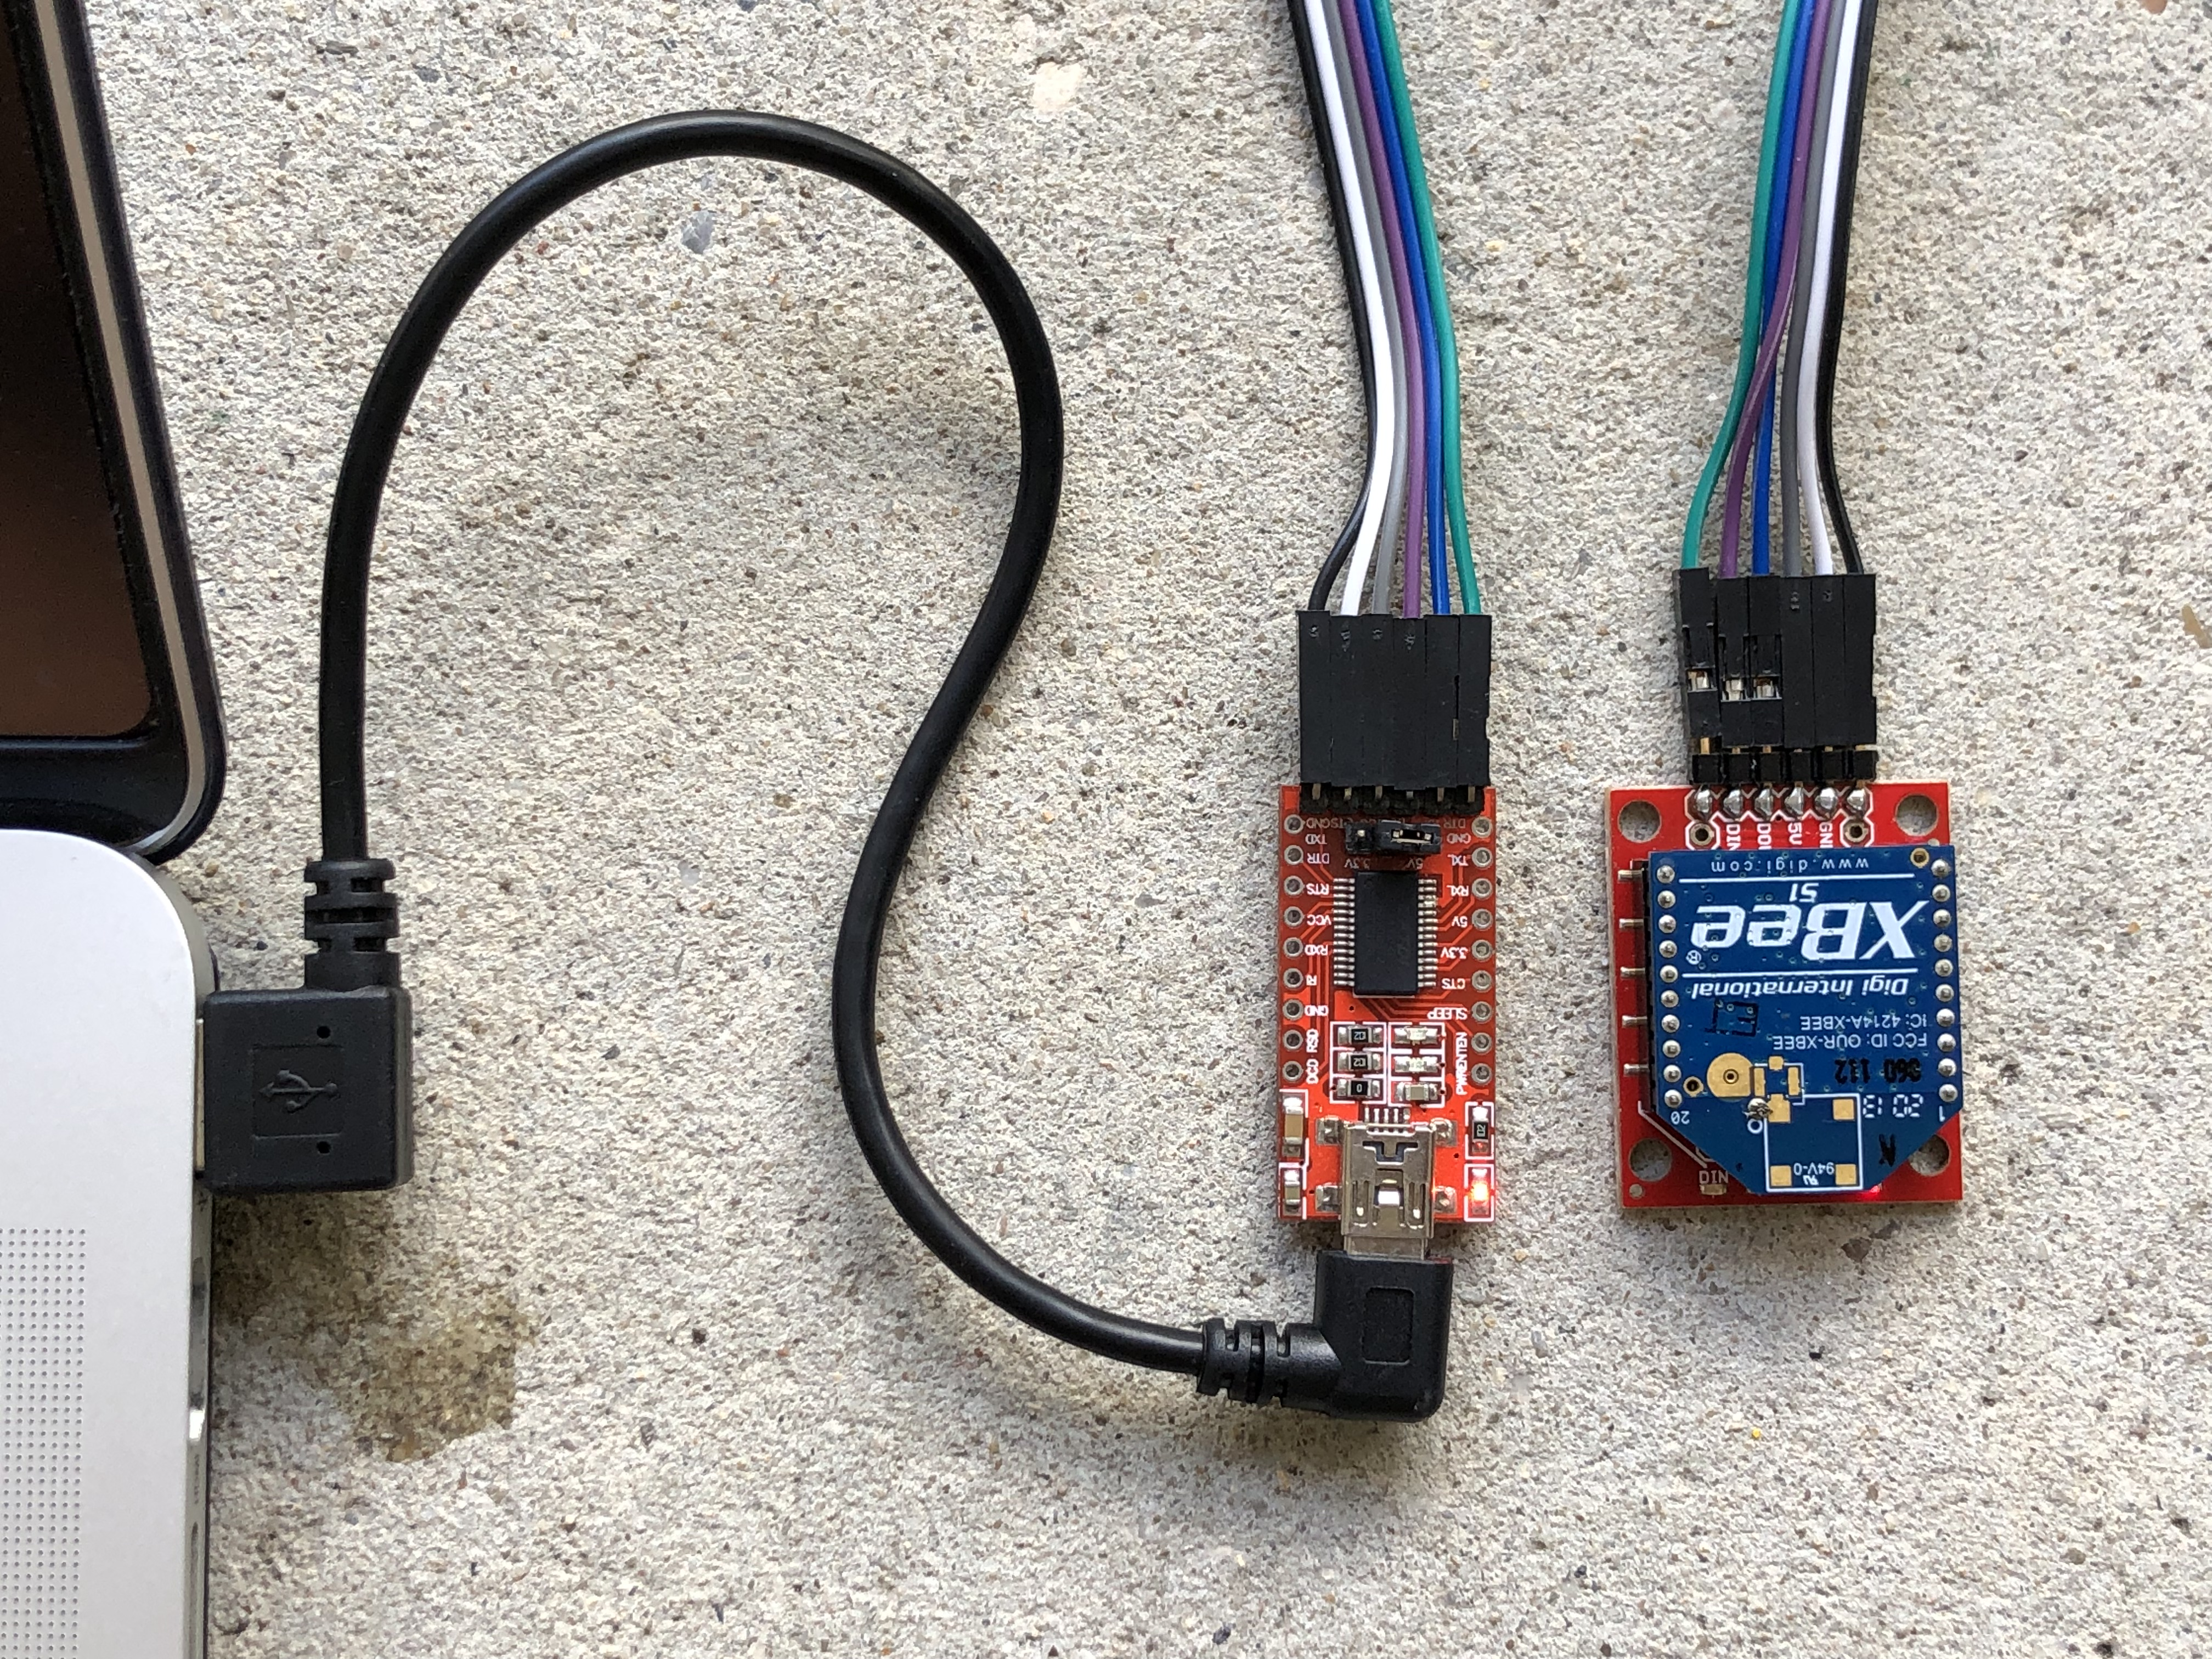
\includegraphics[width=\columnwidth]{comms-hardware.jpg}
\caption{Communications hardware}
\label{commshardware}
\end{figure}

The base station uses an XBee S1 radio on a Sparkfun XBee Explorer Regulated to communicate with the boat. An FTDI232 breakout board allows the computer's USB port to interface with the XBee's UART. This system is shown in Figure \ref{commshardware}.

\subsection{Software}

\begin{figure}[h!]
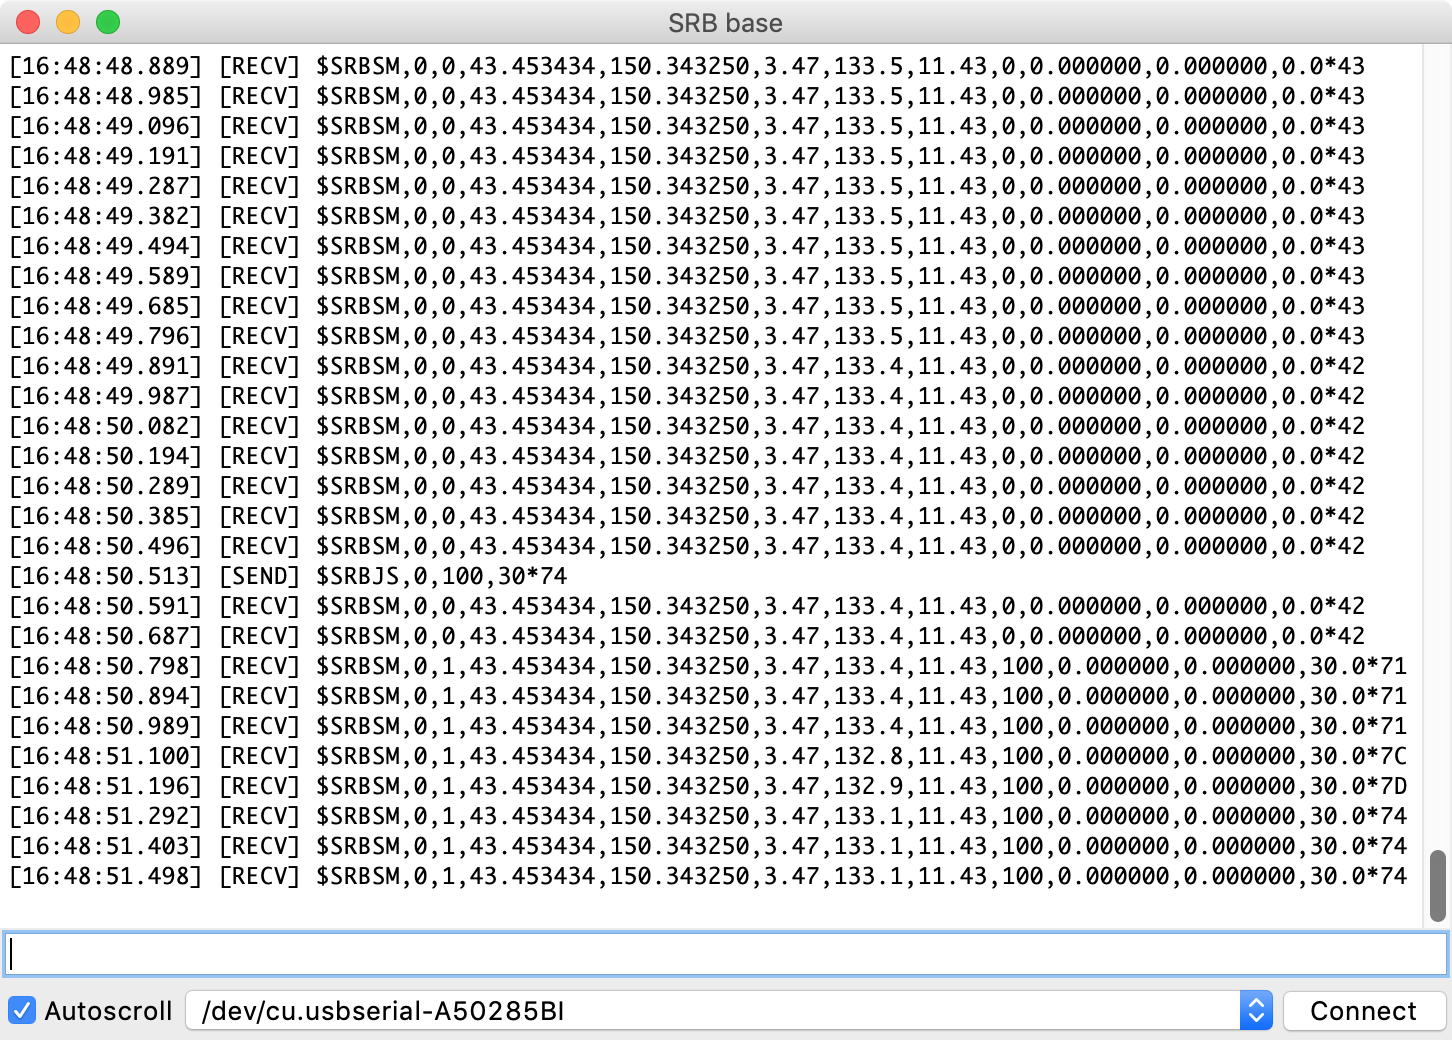
\includegraphics[width=\columnwidth]{srb-base-screenshot.png}
\caption{Screenshot of \texttt{srb-base.py}}
\label{srbbase}
\end{figure}

The Python program \texttt{srb-base.py} was developed to provide a rudimentary graphical interface for the wireless serial connection over XBee. A screenshot of this program is shown in Figure \ref{srbbase}.

The Tkinter interface was modelled on the Arduino IDE's Serial Monitor, but is designed to send NMEA sentences instead of arbitrary text over the serial connection.

"Naked" messages without a leading \texttt{\$} or trailing \texttt{*CS} have these added when they are sent, making it easy to send valid sentences. Incoming messages are validated to ensure the correct syntax and checksum, and invalid sentences are shown in red. The NMEA sentence handler class, \texttt{Nmea}, is separated into the file \texttt{nmea.py}.

All incoming and outgoing messages are logged to the GUI window, terminal window, and a log file in the working directory. The log file includes a comma-separated timestamp at the beginning of each line, allowing the log data to be processed in a makeshift way as a spreadsheet.

The source code for \texttt{srb-base.py} and \texttt{nmea.py} can be found in Appendix A. However, this code is unstable and should not be used as-is, as it was written for testing purposes only.

\section{Testing}
Testing was performed on the power consumption of the boat in a lab setting, as well as the forward speed and turning speed of the boat under typical calm conditions.

\subsection{Power consumption}

\subsubsection{Method}
The boat was elevated in midair on two stands and oriented to face 0 degrees North according to the onboard magnetometers. Two multimeters were connected to the battery, one in parallel measuring the voltage under load, and one in series measuring current.

Starting from an idle state, the message
\begin{center}
\texttt{\$SRBJS,0,<FwdPower>,0*<CS>}
\end{center}
was sent from the base station to the boat, with \texttt{<FwdPower>} as the throttle value being tested. Voltage and current values were recorded once they stabilised. Then, the message
\begin{center}
\texttt{\$SRBJS,0,0,0*46}
\end{center}
was sent from the base station to halt the motors. This was repeated for the throttle levels 0 (idle), 20, 40, 60, 80, and 100.

\subsubsection{Analysis and discussion}
\begin{table}[h!]
\begin{tabu} to \columnwidth {X[c]X[c]X[c]}
\toprule
\textbf{Throttle (\SI{}{\%})} & \textbf{Voltage (\SI{}{V})}  & \textbf{Current (\SI{}{A})} \\ \midrule
0 & & \\ \midrule
20 & & \\ \midrule
40 & & \\ \midrule
60 & & \\ \midrule
80 & & \\ \midrule
100 & & \\ \midrule
\end{tabu}
\caption{Power consumption test results}
\end{table}

\begin{table}[h!]
\begin{tabu} to \columnwidth {X[1.5c]X[c]X[2c]}
\toprule
\textbf{Throttle (\SI{}{\%})} & \textbf{Power (\SI{}{W})}  & \textbf{\SI{11.6}{Ah} runtime (\SI{}{min})} \\ \midrule
0 & & \\ \midrule
20 & & \\ \midrule
40 & & \\ \midrule
60 & & \\ \midrule
80 & & \\ \midrule
100 & & \\ \midrule
\end{tabu}
\caption{Power consumption analysis}
\end{table}


\subsection{Forward speed}

\subsubsection{Method}
The boat was placed in the Brisbane River at a clear, calm location and oriented along the shoreline. A rope was attached to aid retrieval.

Starting from an idle state, the message
\begin{center}
\texttt{\$SRBJS,0,<FwdPower>,<TgtHeading>*<CS>}
\end{center}
was sent from the base station to the boat, with \texttt{<FwdPower>} as the throttle value being tested and \texttt{<TgtHeading>} as the boat's current orientation. After the boat travelled roughly 20 metres, the message
\begin{center}
\texttt{\$SRBJS,0,0,0*46}
\end{center}
was sent back from the base station to halt the motors. The boat was moved back to its starting position. This process was repeated twice for each throttle level being tested.

Messages from the boat were captured into a file using \texttt{srb-base.py}. All messages except for \texttt{SRBSM} were removed by running the terminal command:
\begin{center}
\texttt{\$grep "SRBSM" [logfilename] > results.csv}
\end{center}
which saved the results in a \texttt{.csv} file.

\subsubsection{Analysis and discussion}
\begin{table}[h!]
\begin{tabu} to \columnwidth {X[c]X[c]X[c]X[c]X[c]X[c]X[c]}
\toprule
\multirow{2}{*}{\textbf{Throttle (\SI{}{\%})}} & \multicolumn{3}{c}{\textbf{Accel time (\SI{}{s})}}  & \multicolumn{3}{c}{\textbf{Max speed (\SI{}{\m\per\s})}} \\
& 1 & 2 & avg. & 1 & 2 & avg. \\ \midrule
25 & & \\ \midrule
50 & & \\ \midrule
75 & & \\ \midrule
100 & & \\ \midrule
\end{tabu}
\caption{Forward speed test results}
\end{table}

\begin{figure}[h!]
\centering
\caption{Forward speed vs. time}
\end{figure}

\section{Future development}

\subsection{Boat}
% Voltage/current measurement and logging
% More propellers, 3+ motor omni-drive
% Higher battery capacity for longer runtime
% Structure under boat for stability
% On/off switch

\subsection{Communications}
% Housing for the base station
% Return home mechanism
% Maintain position mechanism

\subsection{Computer vision}
% Been worked on in the past
% Connect this to the comms system
% Brief description of the idea

\section{Conclusion}

\bibliography{bibliography}
\bibliographystyle{IEEEtran}

\clearpage
\appendices

\section{Code}

\srbsource{srb/srb.ino}{C++}
\srbsource{srb/nmea.h}{C++}
\srbsource{srb/nmea.cpp}{C++}
\srbsource{srb/srb_stats.h}{C++}
\srbsource{srb/srb_serial.h}{C++}
\srbsource{srb/srb_serial.cpp}{C++}
\srbsource{srb/srb_gps.h}{C++}
\srbsource{srb/srb_gps.cpp}{C++}
\srbsource{srb/srb_comms.h}{C++}
\srbsource{srb/srb_comms.cpp}{C++}
\srbsource{srb/srb_imu.h}{C++}
\srbsource{srb/srb_imu.cpp}{C++}
\srbsource{srb/srb_motor.h}{C++}
\srbsource{srb/srb_motor.cpp}{C++}
\srbsource{srb/srb_nav.h}{C++}
\srbsource{srb/srb_nav.cpp}{C++}
\srbsource{srb-base/srb-base.py}{Python}
\srbsource{srb-base/nmea.py}{Python}

\onecolumn
\section{Drawings}

\srbdrawing{Top board}{top-board-drawing.pdf}
\srbdrawing{Middle board}{middle-board-drawing.pdf}
\srbdrawing{Bottom board}{bottom-board-drawing.pdf}
\srbdrawing{Motor mount top}{motor-mount-top-drawing.pdf}
\srbdrawing{Motor mount bottom}{motor-mount-bottom-drawing.pdf}

\end{document}